\documentclass[12pt, letterpaper]{article}
\usepackage{graphicx} % Required for inserting images
\usepackage{amsmath}
\usepackage{mdframed}
\usepackage{amssymb}



\title{telegraph equations solved in time with FEM library using MFEM and MFEM ODE Solver Class}
\author{Denis Lachapelle}
\date{February 12, 2026}

\setlength{\parindent}{0pt}

\begin{document}
	
\maketitle

\tableofcontents

\section{Introduction}
This document explains the telegraph equations simulation using finite element method based on MFEM library. The equations are evolved in time by time stepping estimating the partial derivative at each time step of V and I. The stepping method is backward euler in stltfe1d\_05.cpp\\

This document follows stltfe1d\_04 which solve directly y(n+1) in the timeDependentOperator.

\section{Theory}

\subsection{From Telegrah PDE to Matrix form}

The telegraph equations are:

  \begin{equation}\frac{\partial{V(x,t)}}{\partial{x}} + L \frac{\partial{I(x,t)}}{\partial{t}} + R I(x,t) = 0\end{equation}


\begin{equation}\frac{\partial{I(x,t)}}{\partial{x}} + C \frac{\partial{V(x,t)}}{\partial{t}} + G V(x,t) = 0\end{equation}

For now assumes a single line from points a to b. Positive current going from a to b direction.\\

Going to weak form in x domain using different space for V and I, $W^V_i(x)$ for V and $W^I_i(x)$ for I. Note the test functions span the entire domain.

\begin{equation}\int_a^b(\frac{\partial{V(x,t)}}{\partial{x}} + L \frac{\partial{I(x,t)}}{\partial{t}} + R I(x,t))\, W^V_i(x)\, dx = 0\end{equation}

$\forall W^V_i(x)$

\begin{equation}\int_a^b(\frac{\partial{I(x,t)}}{\partial{x}} + C \frac{\partial{V(x,t)}}{\partial{t}} + G V(x,t))\, W^I_i(x)\,dx = 0\end{equation}

$\forall W^I_i(x)$

and then


\begin{equation}
\int_a^b\frac{\partial{V(x,t)}}{\partial{x}} W^V_i(x)\,dx
+ \int_a^b(L \frac{\partial{I(x,t)}}{\partial{t}} +  R I(x,t)) W^V_i(x)\, dx
= 0
\end{equation}



\begin{equation}
\int_a^b\frac{\partial{I(x,t)}}{\partial{x}} W^I_i(x)\, dx
+ \int_a^b(C \frac{\partial{V(x,t)}}{\partial{t}} +  G V(x,t)) W^I_i(x) \, dx
= 0
\end{equation}


Restart with equation 5 and 6 and apply integration by part on $\frac{\partial{I(x,t)}}{\partial{x}}$ of equation 26. so that no BC will be added for the V equation (8).


\begin{equation}
	\int_a^b\frac{\partial{V(x,t)}}{\partial{x}} W^V_i(x)\,dx
	+ \int_a^b(L \frac{\partial{I(x,t)}}{\partial{t}} +  R I(x,t)) W^V_i(x)\, dx
	= 0
\end{equation}



\begin{equation}
	\int_a^b\frac{\partial{I(x,t)}}{\partial{x}} W^I_i(x)\, dx
	+ \int_a^b(C \frac{\partial{V(x,t)}}{\partial{t}} +  G V(x,t)) W^I_i(x) \, dx
	= 0
\end{equation}

Using integration by part on the term $\frac{\partial{I(x,t)}}{\partial{x}}$.

\begin{equation}\int_a^b u(x) v'(x) \, dx = \Big[u(x) v(x)\Big]_a^b - \int_a^b u'(x) v(x) \, dx\end{equation}

The I equation becomes ...

\begin{equation}
	\Big[W^I_i(x) I(x,t) \Big]_a^b
	-\int_a^b I(x,t) \frac{\partial{W^I_i(x)}}{\partial{x}}\, dx
	+ \int_a^b C \frac{\partial{V(x,t)}}{\partial{t}} W^I_i(x)\, dx
	+  \int_a^b G V(x,t) W^I_i(x)\, dx
	= 0
\end{equation}

Then we approximate V and I by summations of possibly different basis function for V $\phi_j$ and I $\psi_j$ as follow:

\begin{equation}
	V(x, t) = \sum_j V_j(t) \phi_j(x), 
	\qquad
	I(x, t) = \sum_j I_j(t) \psi_j(x) 
\end{equation}

And the time derivatives are:

\begin{equation}
	\frac{\partial V(x, t)}{\partial t}
	= \sum_{j} \frac{d V_j(t)}{dt}\,\phi_j(x)
	\qquad
	\frac{\partial I(x, t)}{\partial t}
	= \sum_{j} \frac{d I_j(t)}{dt}\,\psi_j(x)
\end{equation}

Replacing each of $V(x, t), I(x, t), \frac{\partial V(x, t)}{\partial t}$ and $\frac{\partial I(x, t)}{\partial t}$ in equations 7 and 10 we get...

\begin{equation}
	\begin{aligned}
		 \sum_j V_j(t) \int_a^b \frac{\partial{\phi_j(x)}}{\partial{x}}  W^V_i(x) dx \\
		+ L  \sum_j \frac{\partial{I_j(t)}}{\partial t}    \int_a^b \psi_j(x) W^V_i(x) dx 
		+  R  \sum_j I_j(t) \int_a^b \psi_j(x) W^V_i(x) dx \\
		= 0
	\end{aligned}
\end{equation}

and equation 10 becomes ...

\begin{equation}
	\begin{aligned}
		\Big[W^I_i(x) \sum_j I_j(t) \psi_j(x)  \Big]_a^b
		- \sum_j I_j(t) 	\int_a^b \psi_j(x) \frac{\partial{W^I_i(x)}}{\partial{x}} \\
		+ C  \sum_j  \frac{\partial{V_j(t)}}{\partial{t}} \int_a^b \psi_j(x) W^I_i(x) dx
		+ G  \sum_j V_j(t) \int_a^b \phi_j(x) W^I_i(x) dx\\
		= 0
	\end{aligned}
\end{equation}

So now we have two equations (13) and (14) with unknown $V_j(t)$ and $I_j(t)$.\\

The j span the trial functions (Approximating Functions) and the i span the test functions. The equations can be converted in matrix form....

\begin{equation}
	S_V V(t) + L M_V \frac{\partial I(t)}{\partial t} + R M_V I(t) = 
	= 0
\end{equation}

\begin{equation}
	B^b I(t) - B^a I(t)
	- S_I I(t) + C M_I \frac{\partial V(t)}{\partial t} + G M_I V(t) 
	= 0
\end{equation}

One more step to include our particular boundaries.


\begin{equation}
	R_S I_a + V_a = V_S
\end{equation}

The transmission line point b is loaded with a resistor $R_L$.

\begin{equation}
	V_b - R_L I_b = 0
\end{equation}

The boundaries constraints are required just in the 2nd equation.

\begin{equation}
	B^b V(b,t) /R_L - B^a Vs(t) / R_S +  B^a V(a,t) / R_S
	- S_I I(t) + C M_I \frac{\partial V(t)}{\partial t} + G M_I V(t) = 
	= 0
\end{equation}




Where ...

\[S_V = \int_a^b  \frac{\partial \phi_j}{\partial x} W^V_i dx,
\qquad
M_V = \int_a^b \psi_j W^V_i dx\]

\[S_I = \int_a^b \psi_j \frac{\partial W^I_i}{\partial x} dx,
\qquad
M_I = \int_a^b \phi_j W^I_i dx\]

We select trial space for V and I to be H1; later on we may try with I in L2 space.\\

\subsection{Euler Backward}

\begin{equation}
y_{n+1} = y_{n} + \Delta t f(t_{n+1}, y_{n+1})
\end{equation}

Equation 15 and 19 can be written as a single equation with $U(t) = 	\begin{bmatrix}
	I(t) \\
	V(t)
\end{bmatrix} $.

\begin{equation}
	A0\, U(t) + A1\, \frac{\partial U(t)}{\partial t} - A2(t) = 0
\end{equation}


\begin{equation}
	A1\, \frac{\partial U(t)}{\partial t} = - A0\, U(t) + A2(t)
\end{equation}

Where $U(t) = 	\begin{bmatrix}
	I(t) \\
	V(t)
\end{bmatrix} $

$A0 = \begin{bmatrix}
   R M_V & S_V	\\
	- S_I & B^b + B^a + G M_I
\end{bmatrix} $\\

$A1 = \begin{bmatrix}
	L M_V & 0 \\
	0 & C M_I
\end{bmatrix} $\\

$A2(t) = \begin{bmatrix}
	0\\
	 \frac{B^a}{R_s}\, V_s(t)
\end{bmatrix} $\\


MFEM::TimeDependentOperator class implement an operator to implement equation 22 and then MFEM::BackwardEulerSolver class perform the time stepping of $U(t)$.\\

TimeDependentOperator devived class, TelegrapherOperator, will have virtual function ImplicitSolve() implemented since this function is used by BackwardEuler class. This function will return the state vector one time step forward.

Stepping will be done with the BackwardEuler::Step() function.\\








The above formulae shall be used to time step. Rewrite below to match the naming used in the software. Where $I_t$ ant $V_t$ are time derivative.


\begin{equation}
\begin{aligned}
		\begin{bmatrix}
			A11 & 0\\
           01 & A22
		\end{bmatrix}
		*
		\begin{bmatrix}
			I_{t}(t) \\
			V_{t}(t)
		\end{bmatrix}\\
		=
		\begin{bmatrix}
			B11 & B12 \\
			B21 & B22
		\end{bmatrix}
		*
		\begin{bmatrix}
			I(t) \\
			V(t)
		\end{bmatrix}
		+ 
		\begin{bmatrix}
			0 \\
			C2
		\end{bmatrix}
	\end{aligned}
\end{equation}\\


About mfem::BackwardEulerSolver class.

The function mfem::BackwardEulerSolver::Init(TelegrapherOperator) shall be called to associate the TimeDependentOperator to the solver.\\

The function mfem::BackwardEulerSolver::Step(...) is call to step forward in time.




\subsection{MFEM Implementation}

Below are listed the bilinear form and their respective integrators, and the linear form require for signal injection.
\begin{verbatim}	
	A11 = new BilinearForm(FESpace);
	ConstantCoefficient A11Coeff(L);
	A11->AddDomainIntegrator(new MassIntegrator(A11Coeff));
	
	A22 = new BilinearForm(FESpace);
	ConstantCoefficient A22Coeff(C);
	A22->AddDomainIntegrator(new MassIntegrator(A22Coeff));
	
	B11 = new BilinearForm(FESpace);
	ConstantCoefficient B11Coeff(R);
	B11->AddDomainIntegrator(new MassIntegrator(B11Coeff));
	
	B12 = new BilinearForm(FESpace);
	B12->AddDomainIntegrator(new DerivativeIntegrator(one, 0));
	
	B21 = new MixedBilinearForm(FESpace, FESpace);      
	B21->AddDomainIntegrator(new MixedScalarWeakDerivativeIntegrator(one));
	// weak derivative is (-lU, dv/dx)
	
	B22 = new BilinearForm(FESpace);
	ConstantCoefficient B22Coeff(G);
	B22->AddDomainIntegrator(new MassIntegrator(B22Coeff));
	ConstantCoefficient oneOverRsCoeff(1.0/Rs);
	ConstantCoefficient oneOverRlCoeff(1.0/Rl);
	B22->AddBoundaryIntegrator(new BoundaryMassIntegrator(oneOverRsCoeff), *inputBdrMarker);
	B22->AddBoundaryIntegrator(new BoundaryMassIntegrator(oneOverRlCoeff), *outputBdrMarker);
	
	VsRs = new VsRsCoefficient(1.0 / (Rs), SourceFunction);
	C2 = new LinearForm(FESpace);
	C2->AddBoundaryIntegrator(new BoundaryLFIntegrator(*VsRs), *inputBdrMarker);
	
\end{verbatim}


\subsection{Some Simulation Results}
The next two figure show a 1V step tau = 5ns in 100m rg-58 cable driven 50 ohm and a 2 ohm. The first figure (ver 05) is noisier than the second figure (ver 04). In version 04 the solved equation is directly for y(n+1) in ver 05 the solved equation is for dy(n+1)/dt and then y(n+1) is computed from y(n) + deltaT dy(n+1)/dt.  \\
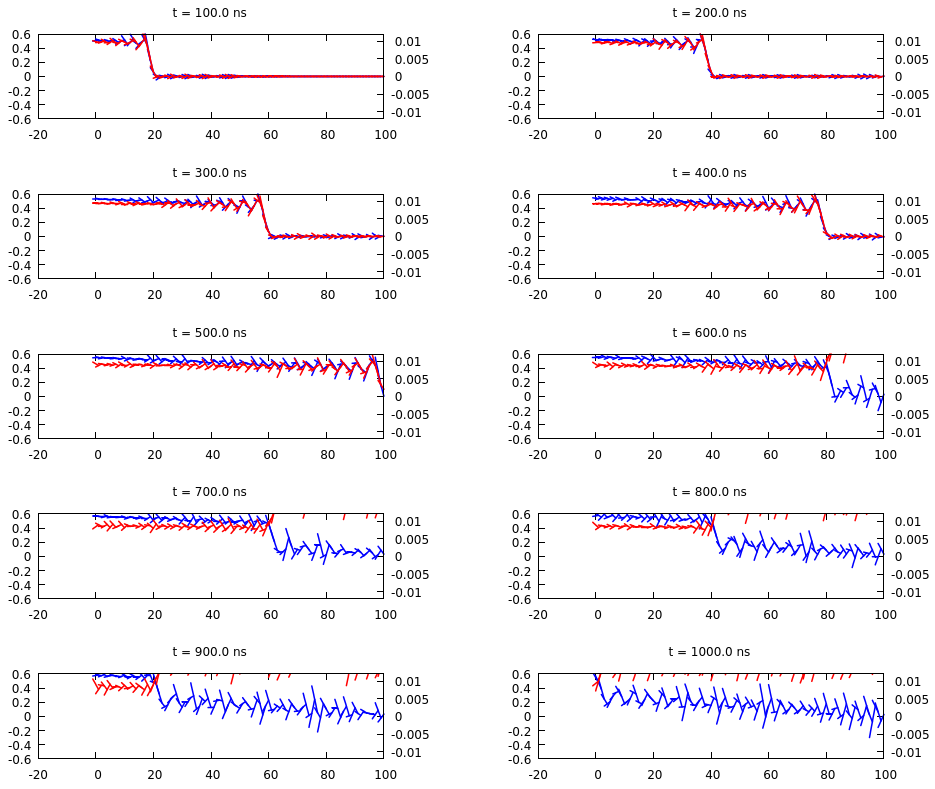
\includegraphics[height=8cm,keepaspectratio]{./step-5.png}\\
\\
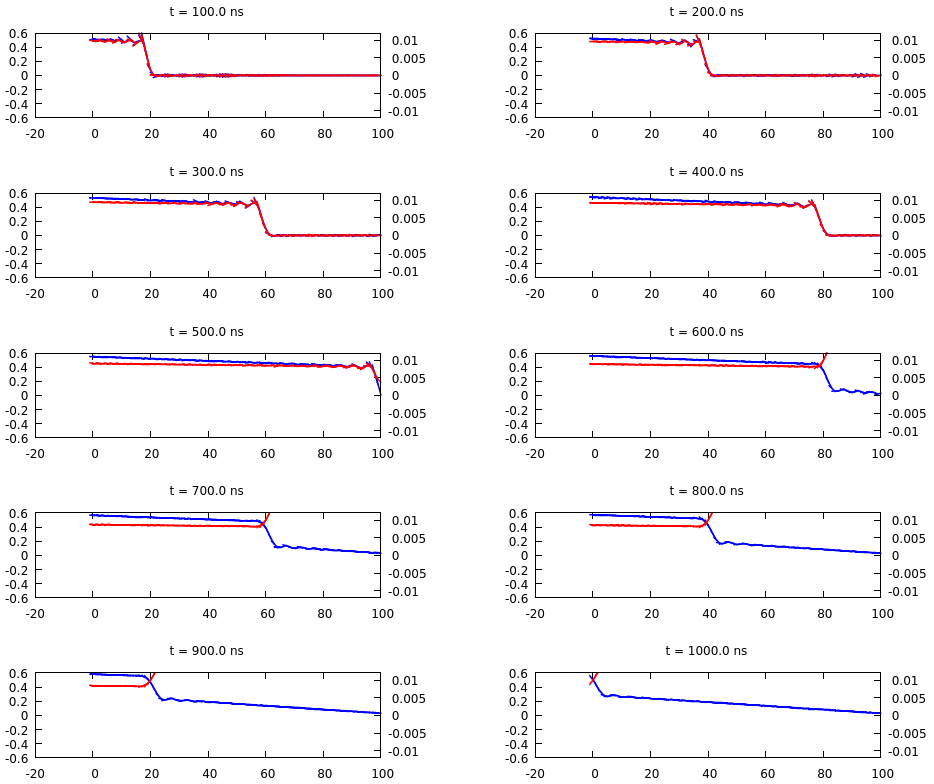
\includegraphics[height=8cm,keepaspectratio]{./step-6.png}\\

\newpage
The next two figures are showing a step signal propagating in a 100m rg-58 cable. The first terminated 50ohm, the second terminated 2ohm.\\
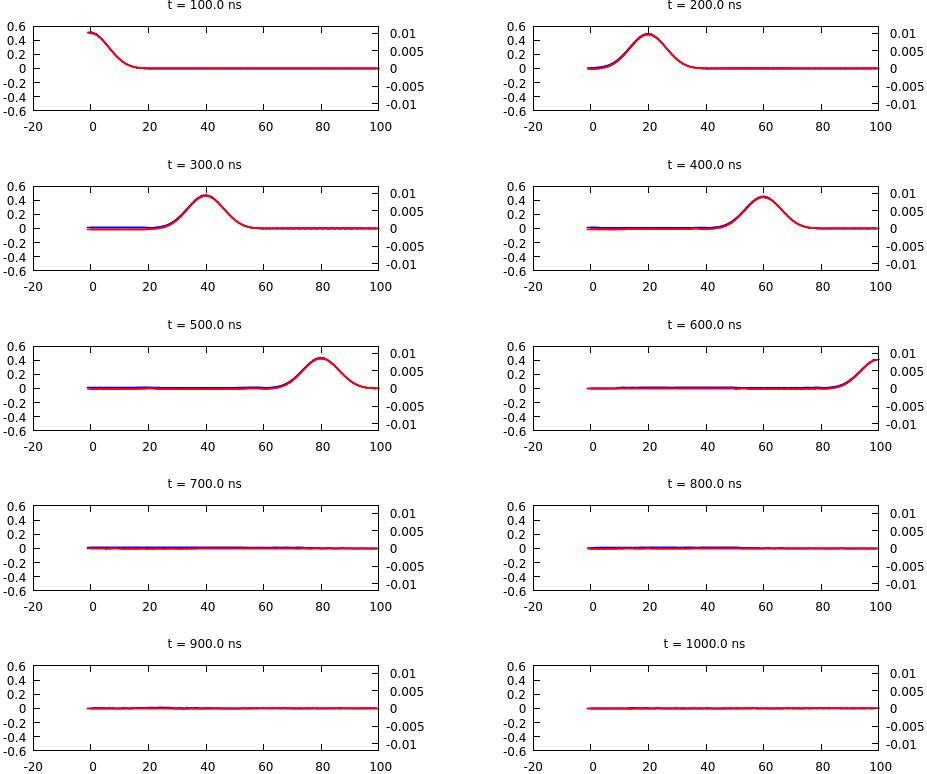
\includegraphics[height=8cm,keepaspectratio]{./pulse-5.png}\\
\\
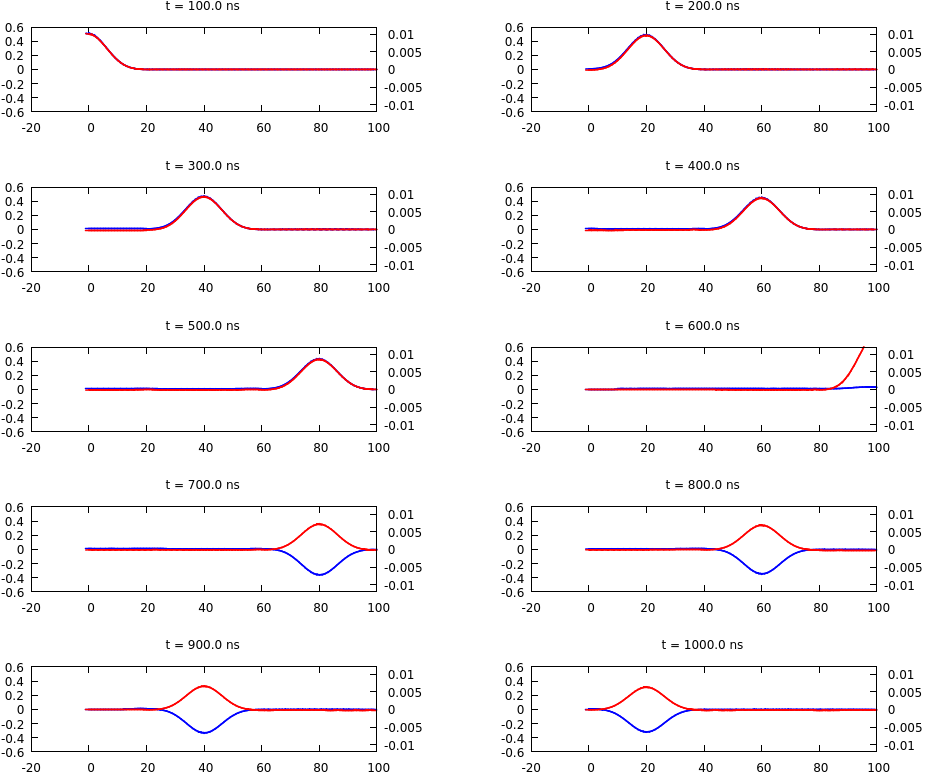
\includegraphics[height=8cm,keepaspectratio]{./pulse-6.png}\\


\newpage
The next figure shows a sine wave propagating through the transmission line, 100m rg-58 cable. The source is 50ohm the load is 2 ohm, we can see the reflection and the current inverting and the attenuation.\\
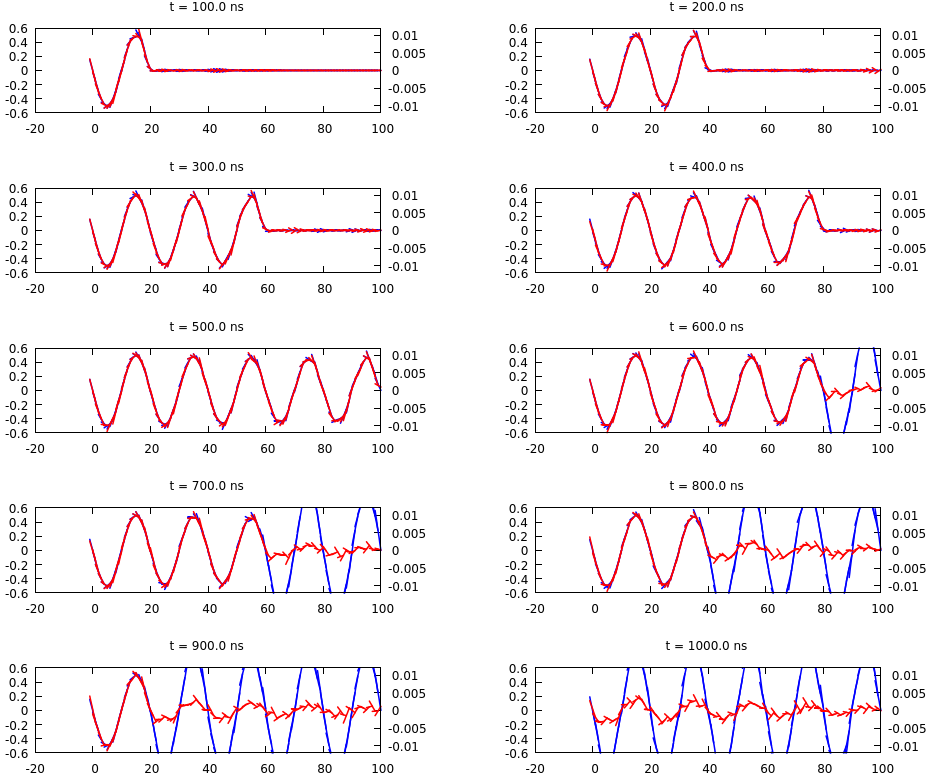
\includegraphics[height=12cm,keepaspectratio]{./sine-5.png}\\

\subsection{What Next}

It would be nice to understand why ver 05 is noisier than ver 04. Ver 05 makes use of mfem class BackwardEulerSolver while version 04 solve directly for y(n+1) within the TimeDependentOperator derived class mult() function.


\end{document}
